
\documentclass[runningheads]{llncs}

% to have bookmarks in pdf
% remove for final version
\usepackage[open,openlevel=5]{bookmark}
\setcounter{tocdepth}{5}

\usepackage{graphicx}
% Used for displaying a sample figure. If possible, figure files should
% be included in EPS format.
%

\graphicspath{{./images/}}

\usepackage{hyperref}
% If you use the hyperref package, please uncomment the following line
% to display URLs in blue roman font according to Springer's eBook style:
\renewcommand\UrlFont{\color{blue}\rmfamily}

%\usepackage{courier}
\usepackage{listings, color}
\hypersetup{
  colorlinks   = true,
  linkcolor  = blue,
  citecolor  = blue,
  urlcolor   = blue
}

% latin modern, no more bitmap fonts in pdf
\usepackage{lmodern}
%\usepackage{newtxtext}
%\usepackage{newtxmath}
\usepackage[zerostyle=b,scaled=.88]{newtxtt}

% nicer bold
\renewcommand{\bfdefault}{b}%


% make paragraph headings bold instead of italics
\renewcommand{\paragraph}{\textbf}%

\definecolor{dkgreen}{rgb}{0,0.6,0}
\definecolor{gray}{rgb}{0.5,0.5,0.5}
\definecolor{mauve}{rgb}{0.58,0,0.82}

\lstdefinestyle{scala}{
  language=scala,
  basicstyle=\footnotesize\ttfamily,
%  basicstyle=\scriptsize\ttfamily, % kai: temporary 
  breaklines=true,
  keywordstyle=\color{blue},
  commentstyle=\color{dkgreen},
  numbers=left,
  %frame=single, % Border around box
  %numbersep=-7pt,
  numberstyle=\color{gray},
  stringstyle=\color{mauve}
}

\lstdefinestyle{stainless}{
  numbers=none,
  breaklines=true,
  breakautoindent=true,
  breakindent=63pt,
  basicstyle=\footnotesize\ttfamily
}
 
\newcommand{\todo}[1]{{\par \color{red}#1}}


\begin{document}

\title{Towards Verifying the Bitcoin-S Library}

\author{Ramon Boss \and Kai Brünnler \and Anna Doukmak}

\authorrunning{R. Boss et al.}
\institute{Bern University of Applied Sciences, CH-2501 Biel, Switzerland
\email{ramon.boss@outlook.com, kai.bruennler@bfh.ch,\\anna.doukmak@gmail.com}}

\maketitle             

\begin{abstract}
  We try to verify some properties of the bitcoin-s library, a Scala
  implementation of parts of the Bitcoin protocol. We use the
  Stainless verifier which supports programs in a subset of Scala
  called \emph{Pure Scala}.  Since bitcoin-s is not written in this
  fragment, we extract the relevant code from it and perform a series
  of equivalent transformations until we arrive at code that we
  successfully verify. In that process we find and fix two bugs in
  bitcoin-s.

\keywords{Bitcoin  \and Scala \and bitcoin-s \and Stainless.}
\end{abstract}



\section{Introduction}

For software handling cryptocurrency, correctness is clearly crucial.
However, even in very well-tested software such as Bitcoin Core,
serious bugs occur. The most recent example is the bug found in
September 2018 \cite{cve201817144} which essentially allowed to
arbitrarily create new coins. Such software is thus a worthwhile
target for formal verification. In this work, we set out to verify
properties of the bitcoin-s library with the Stainless verifier.

\paragraph{The Bitcoin-S Library.} The bitcoin-s library is an
implementation of parts of the Bitcoin protocol in Scala
\cite{BitcoinS:website,BitcoinS:github}. In particular, it allows to
serialize, deserialize, sign and validate Bitcoin transactions. The library
uses immutable data structures and algebraic data types but is not
written with formal verification in mind. According to the website,
the library is used in production, handling significant amounts of
cryptocurrency each day \cite{BitcoinS:website}.

\paragraph{The Stainless Verifier.} Stainless is the successor of the
Leon verifier
\cite{DBLP:conf/ecoop/BlancKKS13,DBLP:conf/pldi/VoirolKK15,DBLP:conf/pldi/BlancK15}
and is developed at EPF Lausanne \cite{Stainless:github}. It is
intended to be used by programmers without training in formal
verification. To facilitate that, it accepts specifications written in
the programming language itself (Scala). Also, it focusses on
counterexample finding in addition to proving
correctness. Counterexamples are useful to programmers while
correctness proofs are not -- correctness is obvious or does not hold,
and often both at the same time.

The example in Figure~\ref{fig:factorial} adapted from the Stainless
documentation \cite{Stainless:documentation} shows how the verifier is
used. Notice how a precondition is specified using \emph{require} and
a postcondition using \emph{ensuring}.

\begin{figure}
\begin{lstlisting}[style=scala]
  def factorial(n: Int): Int = {
      require(n >= 0)
      if (n == 0) {
        1
      } else {
        n * factorial(n - 1)
      }
  } ensuring(res => res >= 0)
\end{lstlisting}
	\caption{Factorial function with specification}
	\label{fig:factorial}
\end{figure}
Our function does not satisfy the specification. An overflow in the
32-bit Int leads to a negative result for the input 17, as Stainless
reports in Figure~\ref{fig:failed}. Changing the type from Int to
BigInt will result in a successful verification.

\begin{figure}
	\centering
		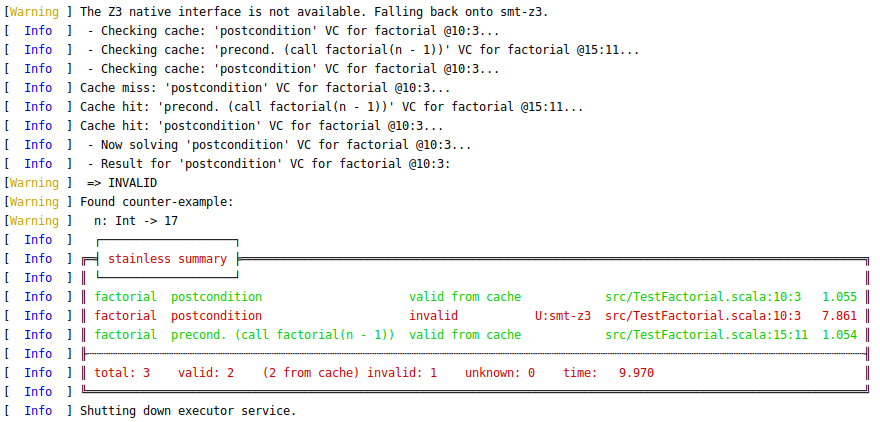
\includegraphics[width=\textwidth]{output1.png}
	\caption{Stainless output for the factorial function}
	\label{fig:failed}
\end{figure}


\paragraph{The Pure Scala Fragment.} The Scala fragment supported by
Stainless is described in the Stainless documentation
\cite{Stainless:documentation} in the section
\href{https://epfl-lara.github.io/stainless/purescala.html}{Pure
  Scala}.

It comprises algebraic data types in the form of abstract classes,
case classes and case objects, objects for grouping classes and
functions, boolean expressions with short-circuit interpretation,
generics with invariant type parameters, default values of function
parameters, pattern matching, local and anonymous classes and more.
In addition to Pure Scala Stainless also supports some imperative
features, such as using a (mutable) variable in a local scope of a
function and while loops. They turn out not to be relevant for the
current work.

What will turn out to be more relevant for us are the Scala features
which Stainless does not support, such as: (concrete) class
definitions, inheritance by objects, abstract type members, and inner
classes in case objects.

Also, Stainless has its own library of some core data types and
functions which are mapped to corresponding data types and functions
inside of the SMT solver that Stainless ultimately relies on. Those
data types in general do not have all the methods of the Scala data
types. For example, the BigInt type in Scala has methods for bitwise
operations while the BigInt type in Stainless does not.

\paragraph{Outline and Properties to Verify.} In the next section we
try to verify the property that a regular (non-coinbase) transaction
can not generate new coins. We call it the \emph{no-inflation
  property}. Trying to verify it, we uncover and fix a bug in the
bitcoin-s library. We then find that there is too much code involved
that lies outside of the supported fragment to currently make this
verification feasible. So we turn to a simpler property to verify. The
simplest possible property we can think of is the fact that adding
zero satoshis to a given amount of satoshis yields the given amount of
satoshis. We call it the \emph{addition-with-zero property} and we try
to verify it in Section~3. Here as well we see that a significant part
of the code lies outside of the supported fragment. We perform a
  series of equivalent transformations on it until we arrive at code that we
  successfully verify. In that process we find and fix a second bug in
  bitcoin-s.


\section{The No-Inflation Property}

\begin{figure}
\begin{lstlisting}[style=scala]
def checkTransaction(transaction: Transaction): Boolean = {
  val inputOutputsNotZero =
    !(transaction.inputs.isEmpty || transaction.outputs.isEmpty)
  val txNotLargerThanBlock = 
    transaction.bytes.size < Consensus.maxBlockSize
  val outputsSpendValidAmountsOfMoney = 
    !transaction.outputs.exists(o =>
      o.value < CurrencyUnits.zero || o.value > Consensus.maxMoney)

  val outputValues = transaction.outputs.map(_.value)
  val totalSpentByOutputs: CurrencyUnit =
    outputValues.fold(CurrencyUnits.zero)(_ + _)
  val allOutputsValidMoneyRange = 
    validMoneyRange(totalSpentByOutputs)
  val prevOutputTxIds = transaction.inputs.map(_.previousOutput.txId)
  val noDuplicateInputs = 
    prevOutputTxIds.distinct.size == prevOutputTxIds.size

  val isValidScriptSigForCoinbaseTx = transaction.isCoinbase match {
    case true =>
      transaction.inputs.head.scriptSignature.asmBytes.size >= 2 &&
        transaction.inputs.head.scriptSignature.asmBytes.size <= 100
    case false =>
      !transaction.inputs.exists(
        _.previousOutput == EmptyTransactionOutPoint)
  }
  inputOutputsNotZero && txNotLargerThanBlock && 
  outputsSpendValidAmountsOfMoney && noDuplicateInputs &&
  allOutputsValidMoneyRange && noDuplicateInputs && 
  isValidScriptSigForCoinbaseTx
}
\end{lstlisting}
  
  \caption{The \texttt{checkTransaction} function}
  \label{fig:checktrans}
\end{figure}


A crucial function for the verification of the no-inflation property
is the \texttt{checkTransaction} function shown in
Figure~\ref{fig:checktrans}. Given a transaction it returns true if
some basic checks succeed, otherwise false. For example, one of those
checks is that both the list of inputs and list of outputs need to be
non-empty.

To better understand the validation of a transaction in bitcoin-s, it
is useful to review how transactions are represented and created.

\paragraph{Creating a Transaction.} The code in this subsection is
adapted from the bitcoin-s documentation. To create a transaction, we
first need some coins -- an unspent transaction output. We could load
an actual unspent transaction output from the bitcoin network, but we
create one manually in order to see this process. So we first create
an (invalid) transaction with one output in Figure~\ref{fig:prevtx}.

\begin{figure}
\begin{lstlisting}[style=scala]
  val privKey = ECPrivateKey.freshPrivateKey
  val creditingSPK = P2PKHScriptPubKey(pubKey = privKey.publicKey)

  val amount = Satoshis(Int64(10000))

  val utxo = TransactionOutput(currencyUnit = amount, scriptPubKey = creditingSPK)

  val prevTx = BaseTransaction(
    version = Int32.one,
    inputs = List.empty,
    outputs = List(utxo),
    lockTime = UInt32.zero
  )
\end{lstlisting}
  
  \caption{Creating a transaction output to spend}
  \label{fig:prevtx}
\end{figure}

We first create a keypair, then a lock script with its public key,
then the amount of satoshis, then a transaction output (utxo) for that
amount and locked with that script. Finally we create a transaction
with that output and no inputs. Of course, that is not a valid
transaction, because it creates coins out of nothing. In particular,
\texttt{checkTransaction(prevTx)} returns false, simply because the list of
inputs is empty.

\begin{figure}
\begin{lstlisting}[style=scala]
  val outPoint = TransactionOutPoint(prevTx.txId, UInt32.zero)

  val utxoSpendingInfo = BitcoinUTXOSpendingInfo(
    outPoint = outPoint,
    output = utxo,
    signers = List(privKey),
    redeemScriptOpt = None,
    scriptWitnessOpt = None,
    hashType = HashType.sigHashAll
  )

  val utxos = List(utxoSpendingInfo)

  val destinationAmount = Satoshis(Int64(5000))

  val destinationSPK = P2PKHScriptPubKey(pubKey = ECPrivateKey.freshPrivateKey.publicKey)

  val destinations = List(
    TransactionOutput(currencyUnit = destinationAmount, scriptPubKey = destinationSPK)
  )

  val feeRate = SatoshisPerByte(Satoshis.one)

  val networkParams = RegTest // some static values for testing

  val txBuilderF: Future[BitcoinTxBuilder] = BitcoinTxBuilder(
    destinations = destinations, 
    utxos = utxos,               
    feeRate = feeRate,           
    changeSPK = creditingSPK,    // where to send the change
    network = networkParams      
  )

  val txF: Future[Transaction] = txBuilderF.flatMap(_.sign)

  val tx: Transaction = Await.result(txF, 1 second)
\end{lstlisting}
  \caption{Creating a transaction}
  \label{fig:tx}
\end{figure}

Now that we have a transaction output, we create a transaction to
spend it in Figure~\ref{fig:tx}. First, we need a reference to an
output of a previous transaction, here called
\texttt{outPoint}. Second, we add some information on how to spend
that output, in particular, how to sign the transaction to allow
this. Now we assemble the list of unspent transaction outputs (utxos),
in our case just one.

We then set the amount of satoshis that we want to spend. The Int64
class aims to emulate a C data type in Scala, and we will look at it
more closely in the next section.

We then create a lock script (\texttt{destinationSPK}) to receive the
coins, create our list of transaction outputs (\texttt{destinations}),
define the fee rate and set some bitcoin network parameters.

Now we create a transaction builder with those data and we tell it to
start signing the transaction in line 34.

Finally, we get the actual signed transaction. We could serialize it
and send it to the Bitcoin network. We can also pass it to the
checkTransaction function, which will return true.

\paragraph{A Bug in the checkTransaction Function.} Note lines 15-17
of the checkTransaction function in Figure~\ref{fig:checktrans}. Here,
value prevOutputTxIds gathers a list of all transaction indentifiers
referenced by the inputs of the current transaction. If the size of
this list is the same as the size of this list with duplicates
removed, we know that no transaction has been referenced twice. This
prevents a transaction from spending two different outputs of the same
previous transaction. The check is too strict: checkTransaction
returns false for valid transactions.

The fix is simple: we perform the duplicate check on the
TransactionOutPoints instead of on their transaction identifiers.  A
TransactionOutPoint contains the txId as well as the output index it
references. Note that TransactionOutPoint is a case class and thus has
a built in == method.

Specifically, we replace lines 15-17 as follows:
\begin{lstlisting}[style=scala, firstnumber=15]
  val prevOutputs = transaction.inputs.map(_.previousOutput)
  val noDuplicateInputs = 
    prevOutputs.distinct.size == prevOutputs.size
\end{lstlisting}


We submitted this fix together with a corresponding unit test to the
bitcoin-s project in a pull request, which has been merged
\cite{BitcoinS:pull435}.


\paragraph{An Attempt at Verification.} Naively trying Stainless on
the entire bitcoin-s codebase results in many errors -- as was to be
expected. We tried to extract only the code relevant to the
no-inflation-property and to verify that. However, even the extracted
code has more than 1500 lines and liberally uses Scala features
outside of the supported fragment.  We tried to transform the code
into the supported fragment, but quickly realized that a better
approach is to first verify a simpler property with less code involved
and later come back to the no-inflation property with more
experience. So we now turn to the addition-with-zero property.




\section{The Addition-with-Zero Property}

It is of course a crucial property we are verifying here: if zero
satoshis were credited to your account, you would not want your
balance to change! It is also the simplest meaningful property to
verify that we can think of. However, the code involved in performing
the addition of two satoshi amounts in bitcoin-s is non-trivial. The
reason for that is a pecularity of consensus code: agreement with the
majority is more important than correctness, whatever correctness
might mean. The most widely used bitcoin implementation by far is the
reference implementation Bitcoin Core, written in C++. For consensus
code, bitcoin-s has little choice but to be in strict agreement with
the reference implementation. To achieve that, it implements C-like
data types in Scala and then implements functionality using those
C-like data types. For example, the Satoshis class, which represents
an amount of satoshis, is implemented using the class Int64 which
aims to represent the C-type \texttt{int64\_t}.

\begin{figure}
\lstinputlisting[style=scala]{../code/addition/src/main/scala/extracted/number/NumberType.scala}
  \caption{Extracted Code from NumberType.scala}
  \label{fig:numbertype}
\end{figure}

\begin{figure}
\lstinputlisting[style=scala]{../code/addition/src/main/scala/extracted/currency/CurrencyUnits.scala}
  \caption{Extracted Code from CurrencyUnits.scala}
  \label{fig:currencyunits}
\end{figure}

\paragraph{Extracting the Relevant Code} The relevant code for the
addition of satoshis is in two files: CurrencyUnits.scala and
NumberType.scala. From those files we removed the majority of the code
because it is not needed for the verification of our property.  For
example, we removed all number types except for Int64 (so Int32,
UInt64, etc.) because they are not used. We also removed the
superclasses Factory and NetworkElement of CurrencyUnit and Number,
respectively, because the inherited members are not used. Also, we
removed all binary operations on Number that are not used, like
subtraction and multiplication. The extracted code is shown in
Figure~\ref{fig:numbertype} and Figure~\ref{fig:currencyunits}.

\paragraph{A Bug in the checkResult Function.} Note the checkResult
function on line 12 and the value andMask on line 23 of
NumberType.scala. The function is intended to catch overflows by
performing a bitwise conjunction of its argument with andMask and
comparing the result with the argument. However, because of the way
Java BigIntegers are represented \cite{wikipedia:twocomp} and because
bitwise operations implicitly perform a sign extension
\cite{java:bigint} on the shorter operand, the function does not
actually catch overflows.

While this is a potentially serious bug, it turns out that checkResult
is only ever called inside a constructor call for a number type (like
Int64) which contains the intended range check, see lines 32-35. The
checkResult function thus can, and should, be removed entirely. The
bitcoin-s developers have acknowledged the bug and we submitted a pull
request to fix it \cite{BitcoinS:pull565}.


\paragraph{Transforming the Code.} We now turn to the list of Scala
features used by the extracted code which are not supported by
Stainless and how to transform the code into the supported fragment.
All transformations are equivalent in the sense that if the
addition-with-zero property holds for the transformed code, then it
also holds for the code before the transformation.

\paragraph{Inheriting Objects.} In both files we have objects
extending the BaseNumbers trait, on lines 30 and 23 respectively,
which Stainless does not support. We simply turn those onjects into
case objects. That transformation is equivalent. Case objects have
various additional properties (for example, being serializable) but
none of our code depends on the absence of any of that.

\paragraph{Abstract Type Members.} In CurrencyUnits.scala on line 6
there is an abstract type that is not supported. Note that we can not
simply replace it by a (supported) type parameter since the
CurrencyUnit class uses one of its implementing classes:
Satoshis. Since the Satoshis class overrides A with Int64 anyway, we
just remove the abstract type declaration and replace A by Int64
everywhere.

\paragraph{Non-Literal BigInt Constructor Argument.} In
CurrencyUnits.scala on line 18 the BigInt constructor is called with a
non-literal argument. As described before, the types in the Stainless
library are more restricted than their Scala library counterparts. In
particular, the Stainless BigInt constructor is restricted to literal
arguments. So we simply replace \texttt{toLong} by
\texttt{underlying.toBigInt}: instead of converting the underlying
Int64 (which in turn has an underlying BigInt) to Long and then back
to BigInt we simply directly return the BigInt. This is an equivalent
transformation: the only thing that might go wrong in the detour via
\texttt{Long} is that the underlying BigInt does not fit into a
Long. However, the only constructor of Int64Impl ensures exactly that
and all functions producing Int64 do so via this constructor.

\paragraph{Self-Reference in Type Parameter Bound.} In
NumberTypes.scala on lines 3 and 19 are classes a type parameter and a
type boundary that contains that typarameter itself. Stainless does
not currently support such self-referential type boundaries. We opened
an issue \cite{Stainless:issue519} on the Stainless repository and the
developers have targeted version 0.4 to support self-referential type
boundaries. Since our code only uses Number with type parameter T
instantiated to Int64, we just remove the type parameter declaration
and replace all its occurrences it by Int64.

\paragraph{Missing Member \texttt{bigInteger} in BigInt.} In NumberType
on line 6 there is a reference to \texttt{bigInteger}. The Scala
BigInt class is essentially a wrapper around
java.math.BigInteger. BigInt has a member bigInteger which is the
underlying instance of the Java class. The Java class has a method
longValueExact which returns a long only if the BigInteger fits into a
long, otherwise throws exception. Stainless does not support Java
classes and in particular its BigInt has no member
bigInteger. However, our code never calls toLong anymore, so we just
remove it.

\paragraph{Type Members.} In NumberType.scala there is a type member
on line 4. Our version of Stainless (0.1) does not support type
members. We just remove the declaration and replace all occurrences of
A with BigInt, since A is never overwritten in an implementing class.
Note that in the mean time Stainless has implemented support for type
members \cite{Stainless:pull470}.  Since version 0.2 verification
should succeed without this change.


\paragraph{Missing Bitwise-And Method on BigInt.} Contrary to Scala
BigInt, the Stainless BigInt class does not support bitwise
operations, in particular not the \&-method used in NumberType.scala
on line 13. However, as described above, the checkResult function is
both broken and redundant, so we remove it and all calls to it.

\paragraph{Inner Class in Case Object.} We have inner classes in
NumberType.scala on line 31 and in CurrencyUnits.scala on line
26. Stainless does not support inner classes in a case object. We just
move the inner classes out of the case objects. They do not interfere
with any other code.

\paragraph{Message Parameter in Require.} The calls of the require
function on lines 32 and 34 in CurrencyUnits.scala have a second
parameter: the error message. Stainless does not support the message
parameter. We simply remove it.

\paragraph{Missing Implicit Long to BigInt Conversion.} The Scala
BigInt class has implict conversions from Long which NumberType.scala
uses on lines 32 and 34 and they are missing in the Stainless
BigInt. Since a BigInt constructor with a Long argument is also
missing, we replace the Long literals by an explicit call to the
BigInt constructor with a literal string argument,
e.g. \texttt{BigInt("-9223...5808")}.


\paragraph{The Specification.} Now that all our code has been
transformed into the supported fragment, we can finally write our
specification, shown in Figure~\ref{fig:spec}, and verify it with
Stainless, as the output in Figure~\ref{fig:result} shows.

\begin{figure}
\lstinputlisting[style=scala, firstline=9, lastline=12, firstnumber=9]{../code/addition/src/main/scala/verified/currency/CurrencyUnits.scala}
\caption{Addition function with specification}
\label{fig:spec}
\end{figure}

\begin{figure}
	\centering
		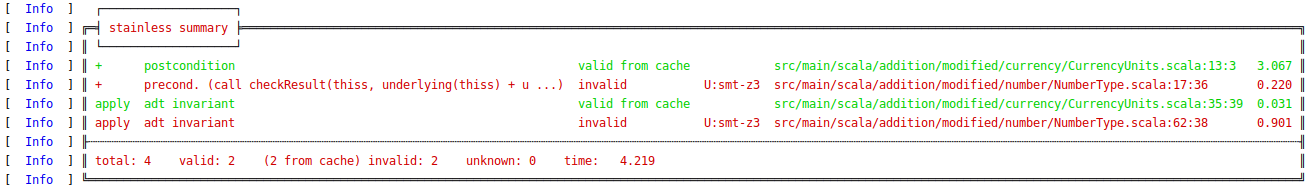
\includegraphics[width=\textwidth]{result_output}
	\caption{Stainless output for the transformed code}
  \label{fig:result}
\end{figure}


\section{Conclusion and Future Work}

We have show
-- bugs (already fixed)
-- suggestions for bitcoin-s

Because of the limitations of the verication tool, we could only
verify a rewritten version of the original Bitcoin-S code.

So code should be written specically with formal verication in mind,

Also, we found that trying to verify code reveals bugs as shown in
section \ref{sec:bugfix}.  Finally, our work led to some feedback to
the Stainless developers to improve the tool.

\bibliographystyle{splncs04}

\bibliography{bibliography}


\clearpage
\appendix





\end{document}
